\subsection{Voltage Level Detector With Hysteresis Applications:}

For the circuit in Figure 3.5.0 we simulate it and captured the results in Figures 4.5.0 and 4.5.1, the results of the measures where registered in table 6:

\begin{figure}[H]
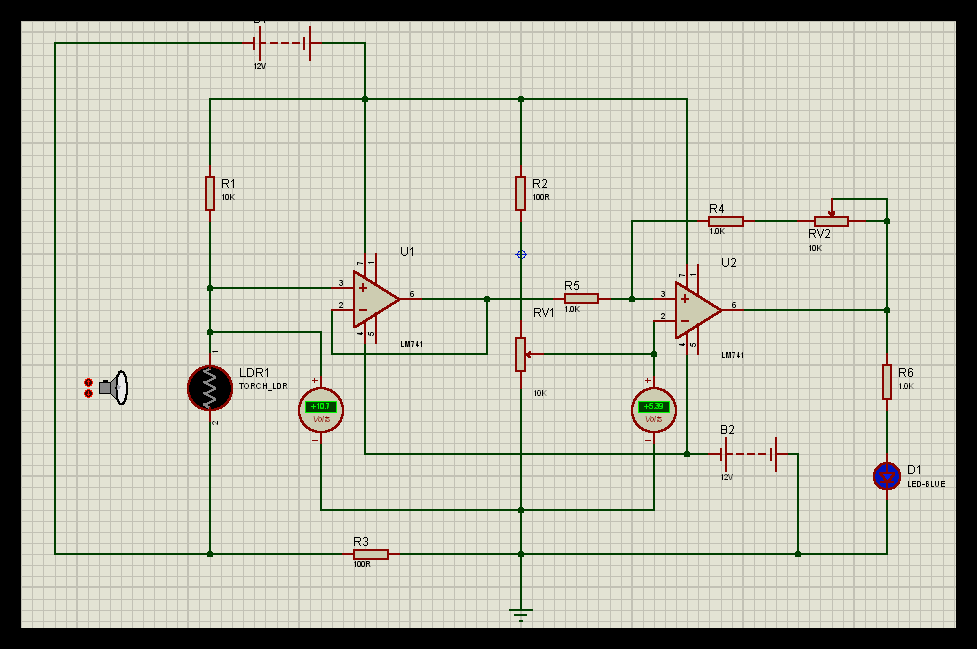
\includegraphics[width = 16.5cm, height = 8cm]{s6-1.png}
\centering \linebreak \linebreak Figure 4.5.0: Level detector with no light near the photocell.
\end{figure} \hfill

\begin{figure}[H]
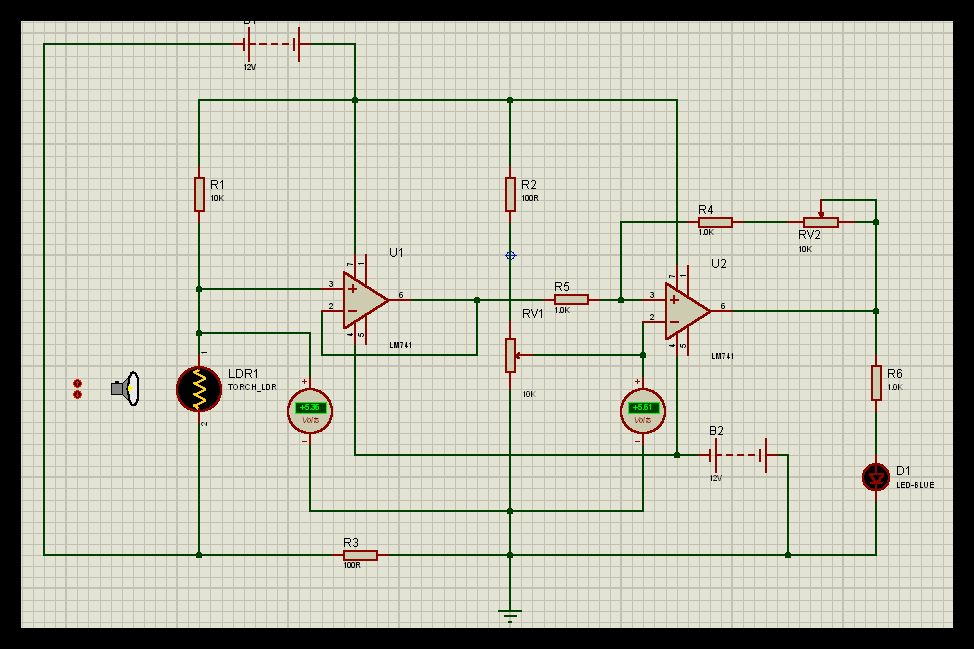
\includegraphics[width = 16.5cm, height = 8cm]{s6-2.png}
\centering \linebreak \linebreak Figure 4.5.1: Level detector with light near the photocell.
\end{figure} \hfill

\begin{center}
\begin{tabular}[.5cm]{c c c}
\toprule
\toprule
\hspace{200pt} & \hspace{100pt} $V_{i}$ \hspace{100pt}  \\
\midrule
\midrule
$V_{ref}$ & 6.39 V \\
\cmidrule{1-2}
Photocell with light & 6.3 V \\
\cmidrule{1-2}
Photocell without light & 10.7 V \\
\bottomrule
\linebreak
\end{tabular}
\linebreak Table 6: Figures 4.5.0 and 4.5.1 voltage levels.
\end{center} \hfill
